\section{Applications}
\begin{frame}
	\frame{\frametitle{Generative Adversarial Networks - Applications}}
\end{frame}

\begin{frame}
	\hyperlink{DCGAN}{
		\begin{figure}[h!]
			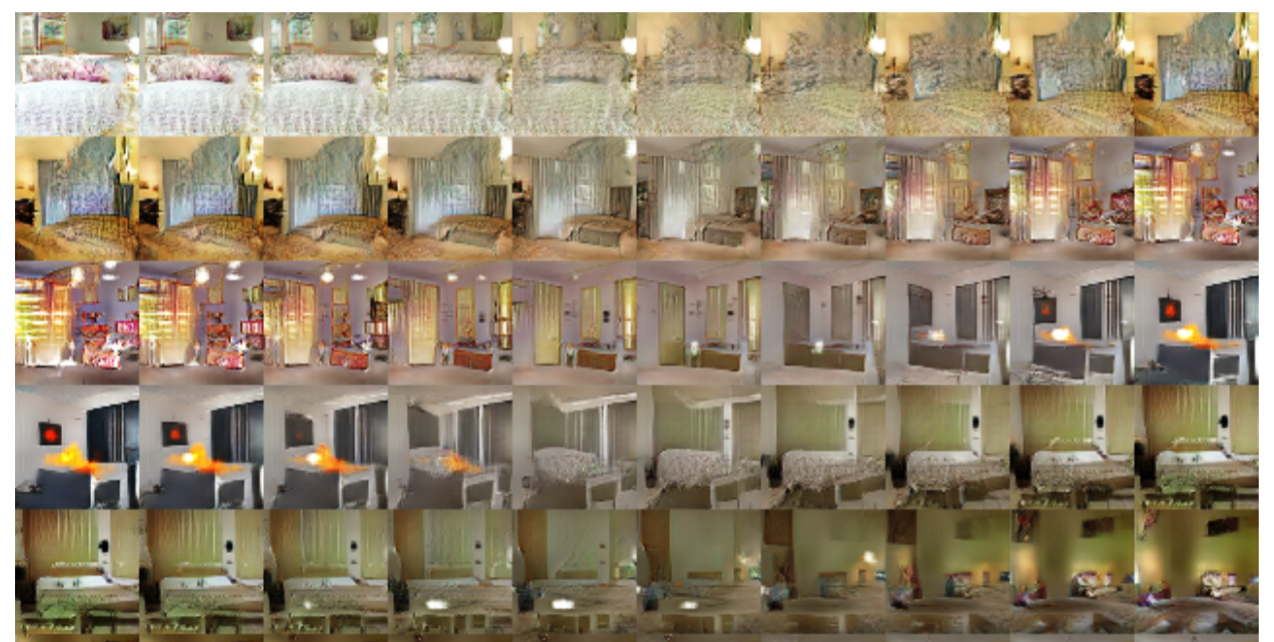
\includegraphics[scale=0.40]{images/Interpolation.png}
		\end{figure}
	}
	\begin{itemize}
		\item In each row the first image was generated by the network by taking a vector $z_1$ as the input and the last images was generated by a vector $z_2$ as the input
		\item All intermediate images were generated by feeding $z$'s which were obtained by interpolating $z_1$ and $z_2$ ($z = \lambda z_1 + (1-\lambda)z_2$)
		\item As we transition from $z_1$ to $z_2$ in the input space there is a corresponding smooth transition in the image space also
	\end{itemize}
\end{frame}

\begin{frame}
	\hyperlink{DCGAN}{
		\begin{figure}[h!]
			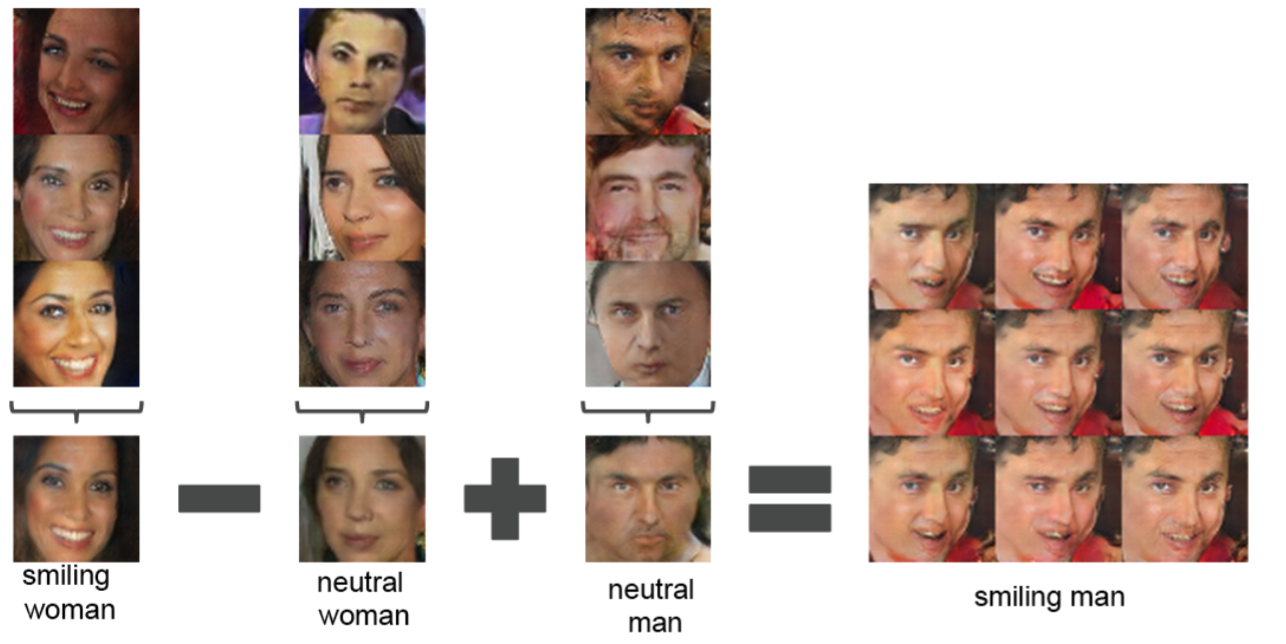
\includegraphics[scale=0.40]{images/Smiling.png}
			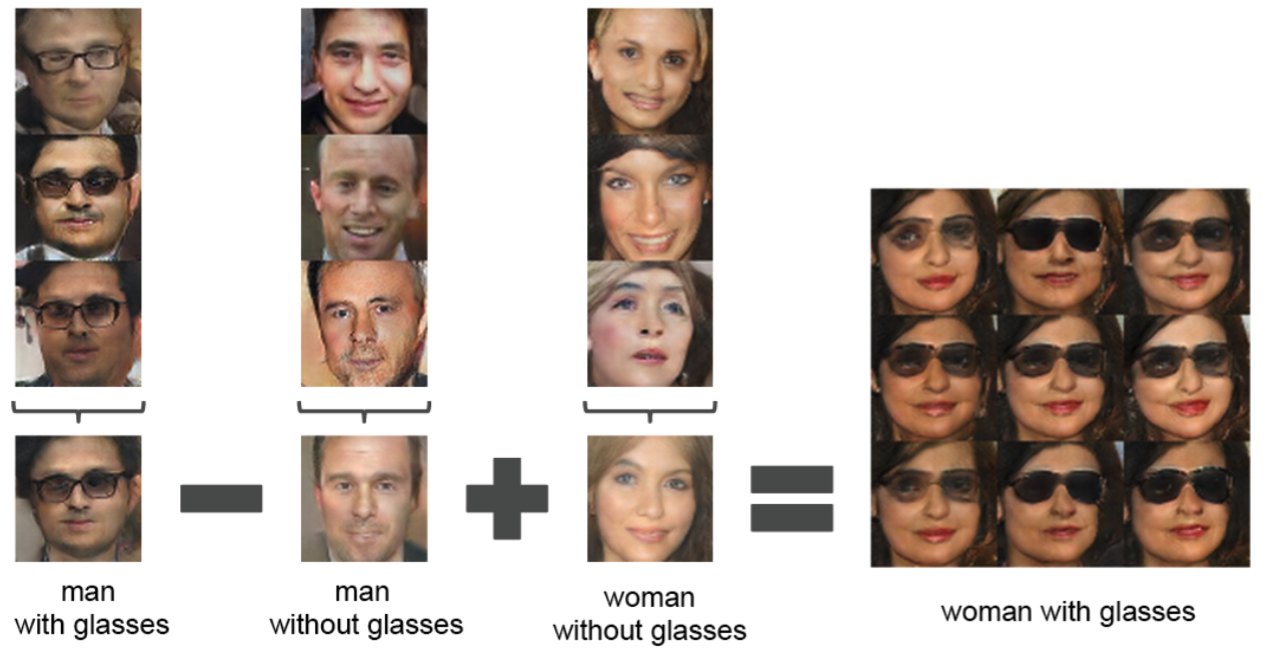
\includegraphics[scale=0.40]{images/Glasses.png}
			\caption{Vector arithmetic for visual concepts (part of figure 7 from the DCGAN paper)}
		\end{figure}
	}
	\begin{itemize}
		\item The first 3 images in the first column were generated by feeding some $z_{11}, z_{12}, z_{13}$ respectively as the input to the generator
		\item The fourth image was generated by taking an average of $z_1 = z_{11}, z_{12}, z_{13}$ and feeding it to the generator
		\item Similarly we obtain the average vectors $z_2$ and $z_3$ for the 2nd and 3rd columns
		\item If we do a simple vector arithmetic on these averaged vectors then we see the corresponding effect in the generated images
	\end{itemize}
\end{frame}

\begin{frame}
	\hyperlink{CAN}{
		\begin{figure}[h!]
			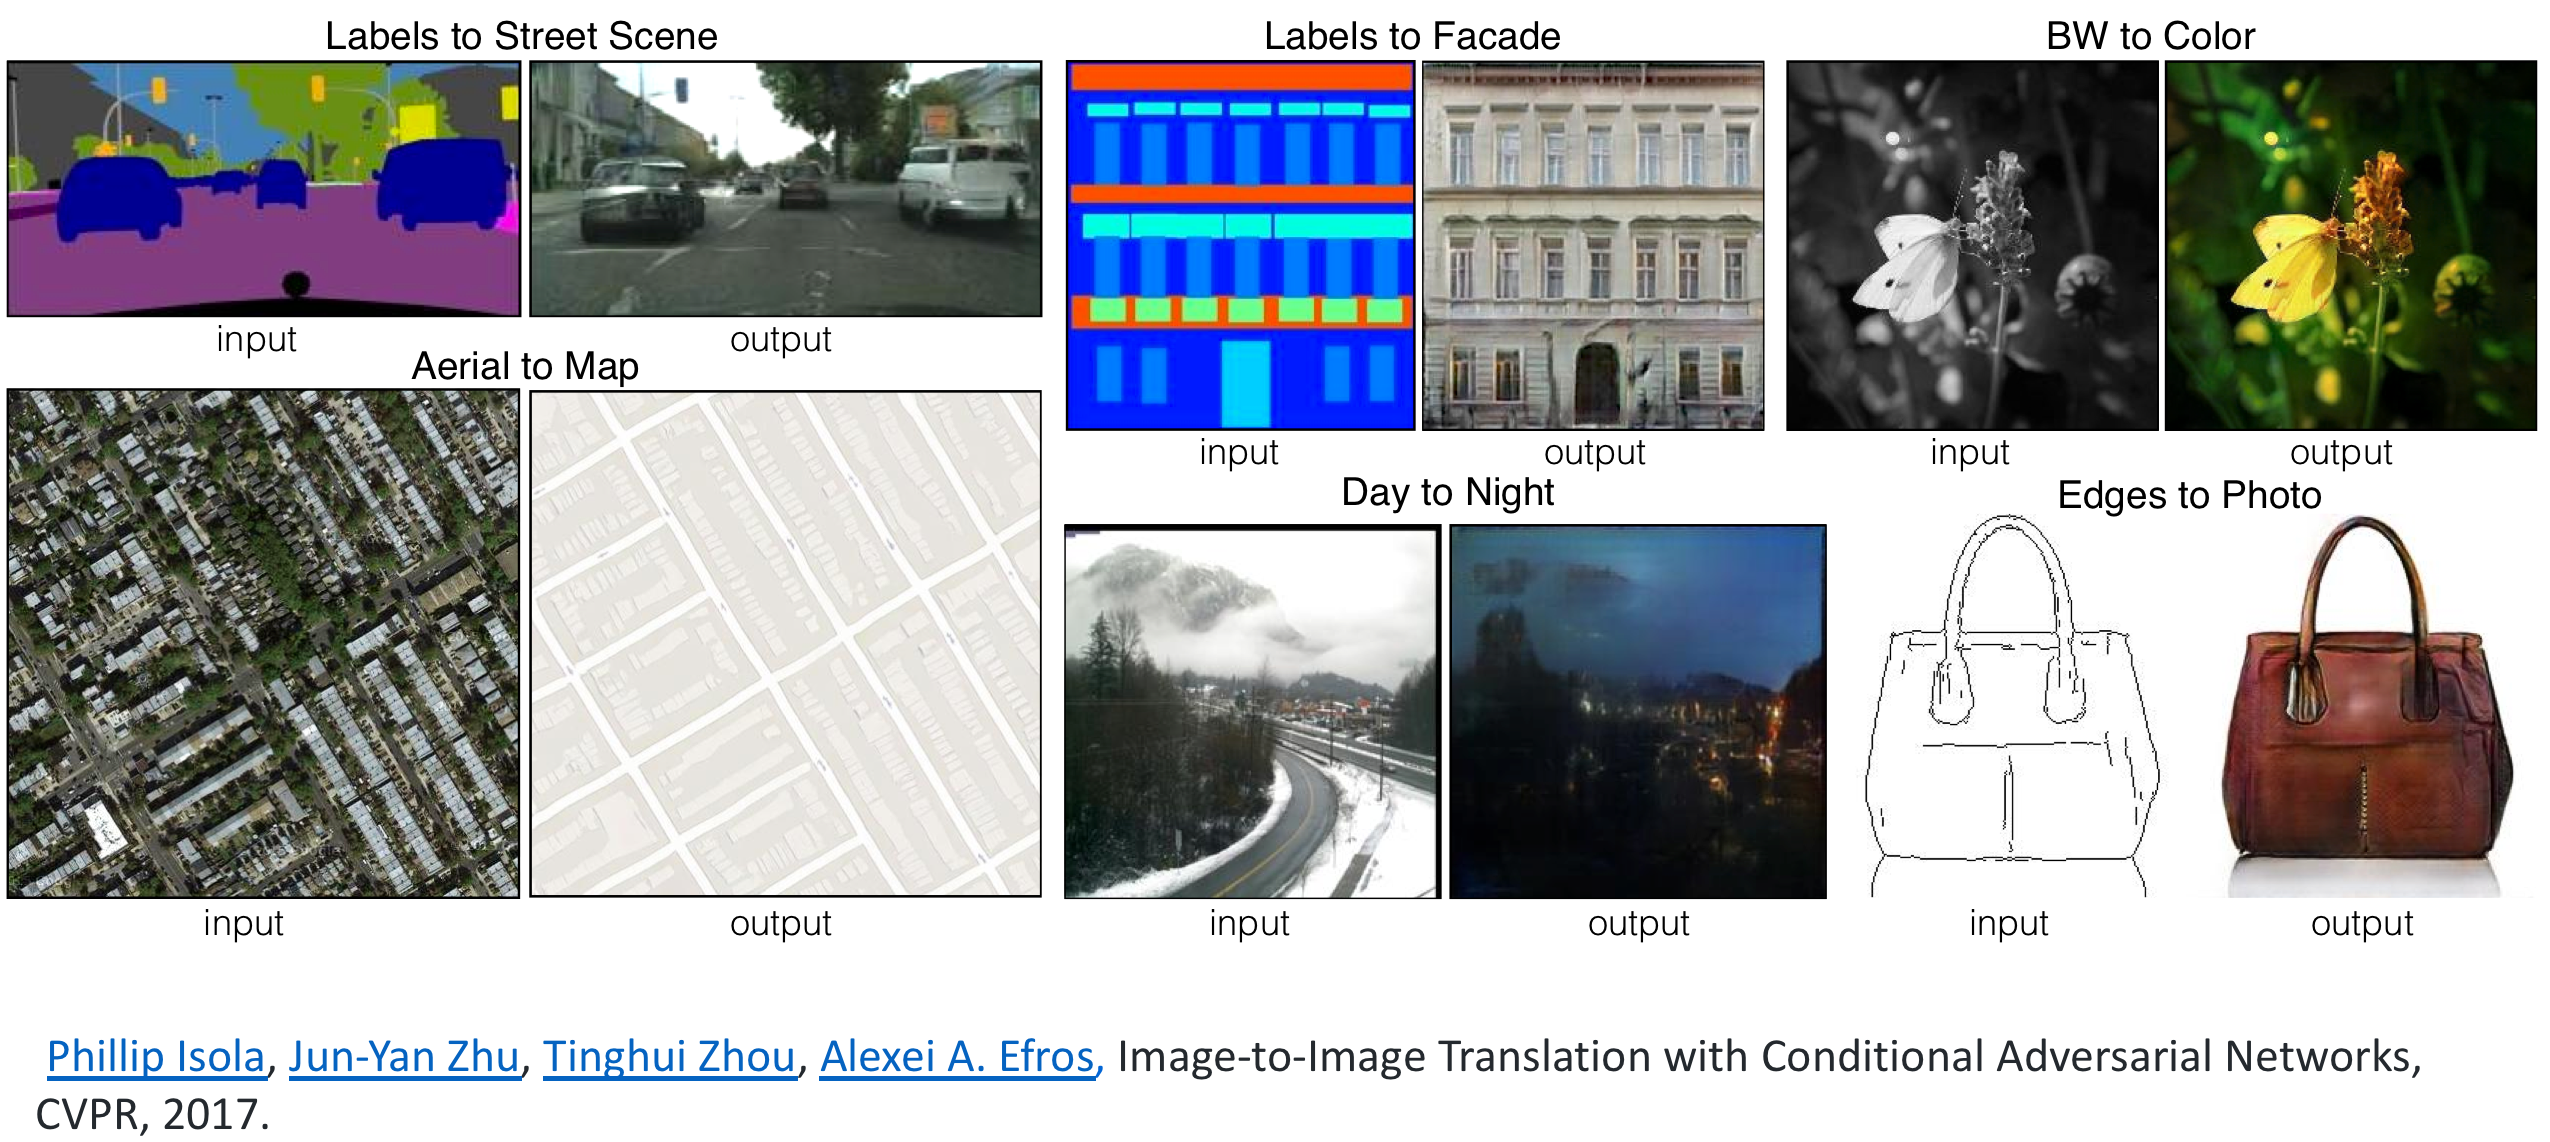
\includegraphics[width=10cm]{images/GAN_Applications.png}
		\end{figure}
	}
\end{frame}

